% Chapter 2

\chapter{Fundamentação Teórica}\label{chap:background}
Ao longo deste capítulo é apresentado o embasamento teórico do projeto, o qual dispõe de pesquisas já realizadas por outros autores sobre os temas propostos envolvendo a área de negócio de aplicação do trabalho, conceitos de alinhamento e estratégias de sistemas, desenvolvimento para plataformas mobile e bancos de dados, os quais servirão de base para o desenvolvimento do trabalho. 

\section{Área de Negócio Aplicada}\label{sec:business}
A área negócio identificada é a tecnologia da informação. A tecnologia da informação é um conjunto de recursos não humanos dedicados ao armazenamento, processamento e comunicação da informação. É a maneira como estes recursos estão organizados em um sistema capaz de executar um conjunto de tarefas \citep{pilla_passaia_2010}.

Já para \cite{rezende_abreu_2003}, tecnologia da informação é tudo aquilo que se refere a todos os equipamentos tecnológicos, envolvendo hardware, software e comunicação, a fim de melhorar a gestão da informação em organizações. Também complementam que as organizações tendem a investir mais neste tipo de tecnologia, devido à valorização que a qualidade da informação como investimento e não como custo.
	
No contexto atual, em que a tecnologia da informação seja capaz de abranger todas, ou a maioria, das atividades desenvolvidas na sociedade, a partir de seus recursos, \cite{ti_albertin_moura} propõem que a tecnologia da informação tem sido destaque como uma das peças mais fundamentais do ambiente corporativo, sendo utilizado em larga escala tanto em nível estratégico como operacional. \\

Em contato com a empresa notou-se que, atualmente, os chamados de suporte são realizados a partir de mensagens diretas com o profissional responsável pela infraestrutura de TI da empresa ou por e-mail. Tal comportamento acaba atrapalhando a comunicação interna em alguns casos, pois os meios de comunicação para discussão de outros problemas acabam sendo confundidos e misturados com os pedidos de suporte.

\section{ALINHAMENTO E ESTRATÉGIAS DOS SISTEMAS}\label{sec:rw}
Neste capítulo, são abordados os assuntos referentes à alinhamento e estratégias de sistemas, cadeira estudada durante o período de desenvolvimento deste trabalho. Alinhamento e estratégias de sistemas tem o objetivo de provocar uma visão ampla sobre os conceitos e principais características a serem consideradas para a implementação das melhores práticas de Gestão de Serviços de TI, tradução livre para o termo ITIL, e também aborda os desafios e benefícios da sua aplicação prática. Respectivamente, são colocados os itens de Gerenciamento de Serviços de TI, com foco em ITIL na área de gerenciamento de serviços de TI.

\subsection{Gerenciamento de Serviços de TI}
Segundo \cite{gerenciamentoti_itil_magalhaes_pinheiro} independentemente do modelo de negócios da organização, a infraestrutura de TI deve possuir um modelo de gerenciamento de serviços compatível com os serviços necessários para a continuidade da área, bem como da organização como um todo.

De toda forma, o gerenciamento de serviços de TI é tido como uma ferramenta fundamental para a constante melhoria dos serviços de TI, objetivando sempre obter o melhor custo/benefício, se apresentando de forma confiável para o usuário.
\subsubsection{Serviços de TI}
Conforme \cite{mildner_2009} \textit{apud} \cite{gerenciamentoti_itil_magalhaes_pinheiro}, um serviço de TI pode ser definido como um conjunto de recursos de TI e “não-TI”, porém mantidos por um provedor de TI. Esse provedor, por sua vez, tem o objetivo de satisfazer uma ou mais necessidades de um cliente, também suportando os objetivos estratégicos do seu negócio, assim, podendo ser percebido pelo cliente como um todo de forma coerente.
    
No guia ITIL, um serviço de TI é definido como um ou mais sistemas que habilitam um processo de negócio. Portanto é necessário considerar que um sistema de TI é uma combinação envolvendo hardware, software, facilidades, processos e pessoas.
\subsubsection{ITIL}
O ITIL surgiu na década de 80 no Reino Unido sob o nome de \textit{Government Information Technology Infraestructure Method} (GITIM), com a finalidade de suprir as necessidades do governo na padronização de práticas e serviços de TI. Serviu como um guia de boas práticas, e de tal forma, demais organizações demonstraram interesse em utilizá-lo. Sendo assim, em 1989 passou a ser chamado de \textit{Information Technology Infraestructure Library} (ITIL), com a proposta de que fosse um conteúdo aberto a quem tivesse interesse \citep{freitas_2013}.

O ITIL agrega em sua síntese cinco processos operacionais que são: gerenciamento de configuração, gerenciamento de incidentes, central de serviços, gerenciamento de problemas, gerenciamento de mudanças e gerenciamento de liberações. Além disso, agrega cinco processos táticos, gerenciamento de nível de serviço, gerenciamento de disponibilidade, gerenciamento de capacidade, gerenciamento financeiro dos serviços de TI e gerenciamento da continuidade dos serviços de TI \citep{vanharen_2006}.

O principal objetivo do ITIL, observado como um framework, é disponibilizar um conjunto de boas práticas para gerenciar serviços de TI. Essas práticas foram testadas e comprovadas que podem ser edificadoras para empresas leigas em TI,  como em empresas onde já existem diversas operações relacionadas a área ou que pretendem empreender em melhorias nas operações \citep{ogc_itil}.

\subsubsection{Gerenciamento de incidentes e abertura de chamados}
A área de suporte a serviços citada no ITIL aborda cinco processos que se relacionam entre si. Desta maneira, é possível  ajudar a manter a entrega de serviços ao se concentrar nas atividades diárias do suporte a serviços de TI \citep{vanharen_2006}.

\subsubsection{Central de Serviços}
Ainda em termos de área de suporte há a central de Serviços, a qual serve como ponto inicial de contato dos usuários com a área ou organização de TI. Em algumas edições mais antigas do guia ITIL, é possível encontrar o nome Central de assistência, a qual tinha as tarefas de registrar, resolver e monitorar os problemas. No entanto, a Central de Serviços tem um viés mais amplo, tais como receber requisições de mudanças ou realizar atividades que pertencem a vários processos

Ainda de acordo com \citet{vanharen_2006}, os processos da  área de suporte a serviços são: gerenciamento de incidentes, gerenciamento de problemas, gerenciamento de configurações, gerenciamento de mudanças e gerenciamento de liberações e operação da central de serviços.

\subsubsection{Gerenciamento de Incidentes}
O processo de gerenciamento de incidentes propende-se a solucionar o incidente rapidamente e imediatamente após isso restaurar os serviços que foram afetados. Os incidentes devem ser registrados e por consequência disso, a qualidade da descrição dos registros pode determinar a eficiência desse processo e outros \citep{ogc_itil}. 

\subsubsection{Gerenciamento de problemas}
O gerenciamento de problemas é o processo responsável por identificar a causa-raiz quando se suspeita de algum problema. Pode-se suspeitar de um problema a partir do momento em que há incidentes, todavia é sempre que possível antecipar-se aos problemas de forma a evitar impactos \citep{ogc_itil}. 

Uma vez que tenham sido identificadas as causas, e que também se tenha identificada uma solução de contorno, o problema deve ser categorizado como um erro conhecido e, então toma-se uma decisão com a relação a realização, ou não, de uma correção permanente para evitar novos incidentes. A correção do problema se da através de uma RDM (requisição de mudança).

Em um caso que não seja possível encontrar uma justificativa para a correção do problema, porém com uma solução temporária ou ainda uma alternativa permanente, o problema continua sendo classificado como um erro conhecido.

\subsubsection{Gerenciamento de configurações}
O processo de Gerenciamento de configurações visa tratar do controle de padronização, identificação de componentes, gerenciamento dos detalhes sobre componentes em uma infraestrutura de TI \citep{ogc_itil}.

\subsubsection{Gerenciamento de mudanças}
O processo de gerenciamento de mudanças cognomina-se da aprovação e implementação das mudanças na infraestrutura de TI com o objetivo de avaliar as mudanças garantindo que as mesmas possam ser implementadas afetando minimamente os serviços de TI \citep{ogc_itil}. 

\subsubsection{Gerenciamento de Liberações e operação da central de serviços}
Antes de definir o processo, se faz necessário definir a liberação em si, e uma liberação, segundo \citet{vanharen_2006}, é um conjunto de itens de configuração que são testados e introduzidos no ambiente de produção.

O principal objetivo do processo de gerenciar liberações é garantir a implementação das liberações, para assim ter a capacidade de certificar que somente são fornecidas versões corretas e autorizadas de \textit{software} e \textit{hardware}.

\section{Desenvolvimento de Software}
No quesito de desenvolvimento de software, serão aplicados os paradigmas previstos em ementa da cadeira de Linguagem de Programação III. O conteúdo propõe o desenvolvimento de aplicativos mobile. Ao decorrer do capítulo serão abordados os tópicos de sistemas operacionais mobile, arquitetura de serviços mobile, linguagem de programação e bancos de dados
\pagebreak
\subsection{Sistemas Operacionais}
Para \citet{so_tanembaum}, É difícil afirmar com absoluta certeza o qual o conceito primário de um sistema operacional, pois além de também atua como o software que opera no núcleo. Em geral, sistemas operacionais realizam basicamente duas funções que não são relacionadas, uma delas é fornecer um conjunto de recursos abstratos limpo, como programas e aplicativos, e gerenciar os recursos de hardware em questão. Em outras palavras, SOs na verdade fazem transformações hardware em abstrações entendíveis ao usuário final. A figura \ref{fig:so_abstracoes} exemplifica as abstrações de sistemas operacionais em níveis de Hardware, SO e aplicativos.

\begin{figure}[htb]
     \caption {Abstrações de sistemas operacionais}
     \centering
     \begin{frame}{
     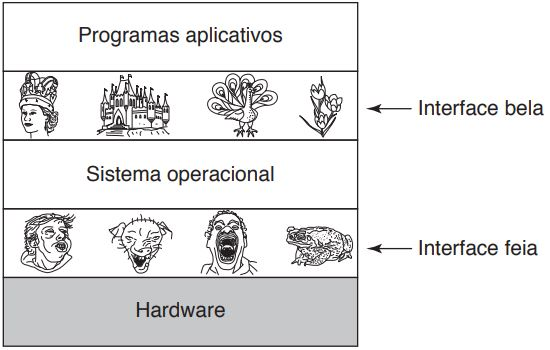
\includegraphics [scale=0.7,]{img/so_tanembaum.JPG}}
     \end{frame}
     \label{fig:so_abstracoes}
     \source{Retirado de \cite{so_tanembaum}.}
 \end{figure}

\subsection{Sistemas Operacionais Mobile}

Os SO mobile levam o mesmo conceitos que um SO tradicional, porém são aplicados em dispositivos móveis, como \textit{smartphones} e \textit{tablets}. Levam destaque, hoje, os aparelhos com suporte a \textit{touchscreen} e sem nenhum ou com poucos botões físicos. Os principais SO mobile, atualmente, são o Android, desenvolvido pela Google, e o Ios, que é propriedade da Apple. 

O Android é um sistema operacional projetado para executar em dispositivos móveis e é baseado no kernel Linux, de forma a introduzir alguns conceitos para o próprio kernel do Linux, usando a maioria dos mecanismos clássicos do Linux como processos, IDs de usuário, memória virtual, sistemas de arquivos e escalonamento, porém muitas vezes de maneira bem diferente da maneira para qual foram projetados. \citep{so_tanembaum}. 

A figura \ref{fig:so_arq_dev_android} exibe a pilha de software do android para exemplificar as camadas do sistema operacional. No nível mais baixo há o gerenciamento de energia, sobreposto por um kernel linux com seus drivers. Acima do kernel linux existe a camada de abstração de hardware, seguida pelas camadas de biblioteca de linguagem Android nativa, a a qual trabalha lado a lado com as bibliotecas de C/C++ nativas. Acima dessas duas camadas localiza-se a API do Java e no nível mais alto os aplicativos instalados no aparelho.

\begin{figure}[htb]
    \caption{Pilha de software do Android}
    \centering
    \begin{frame}{
    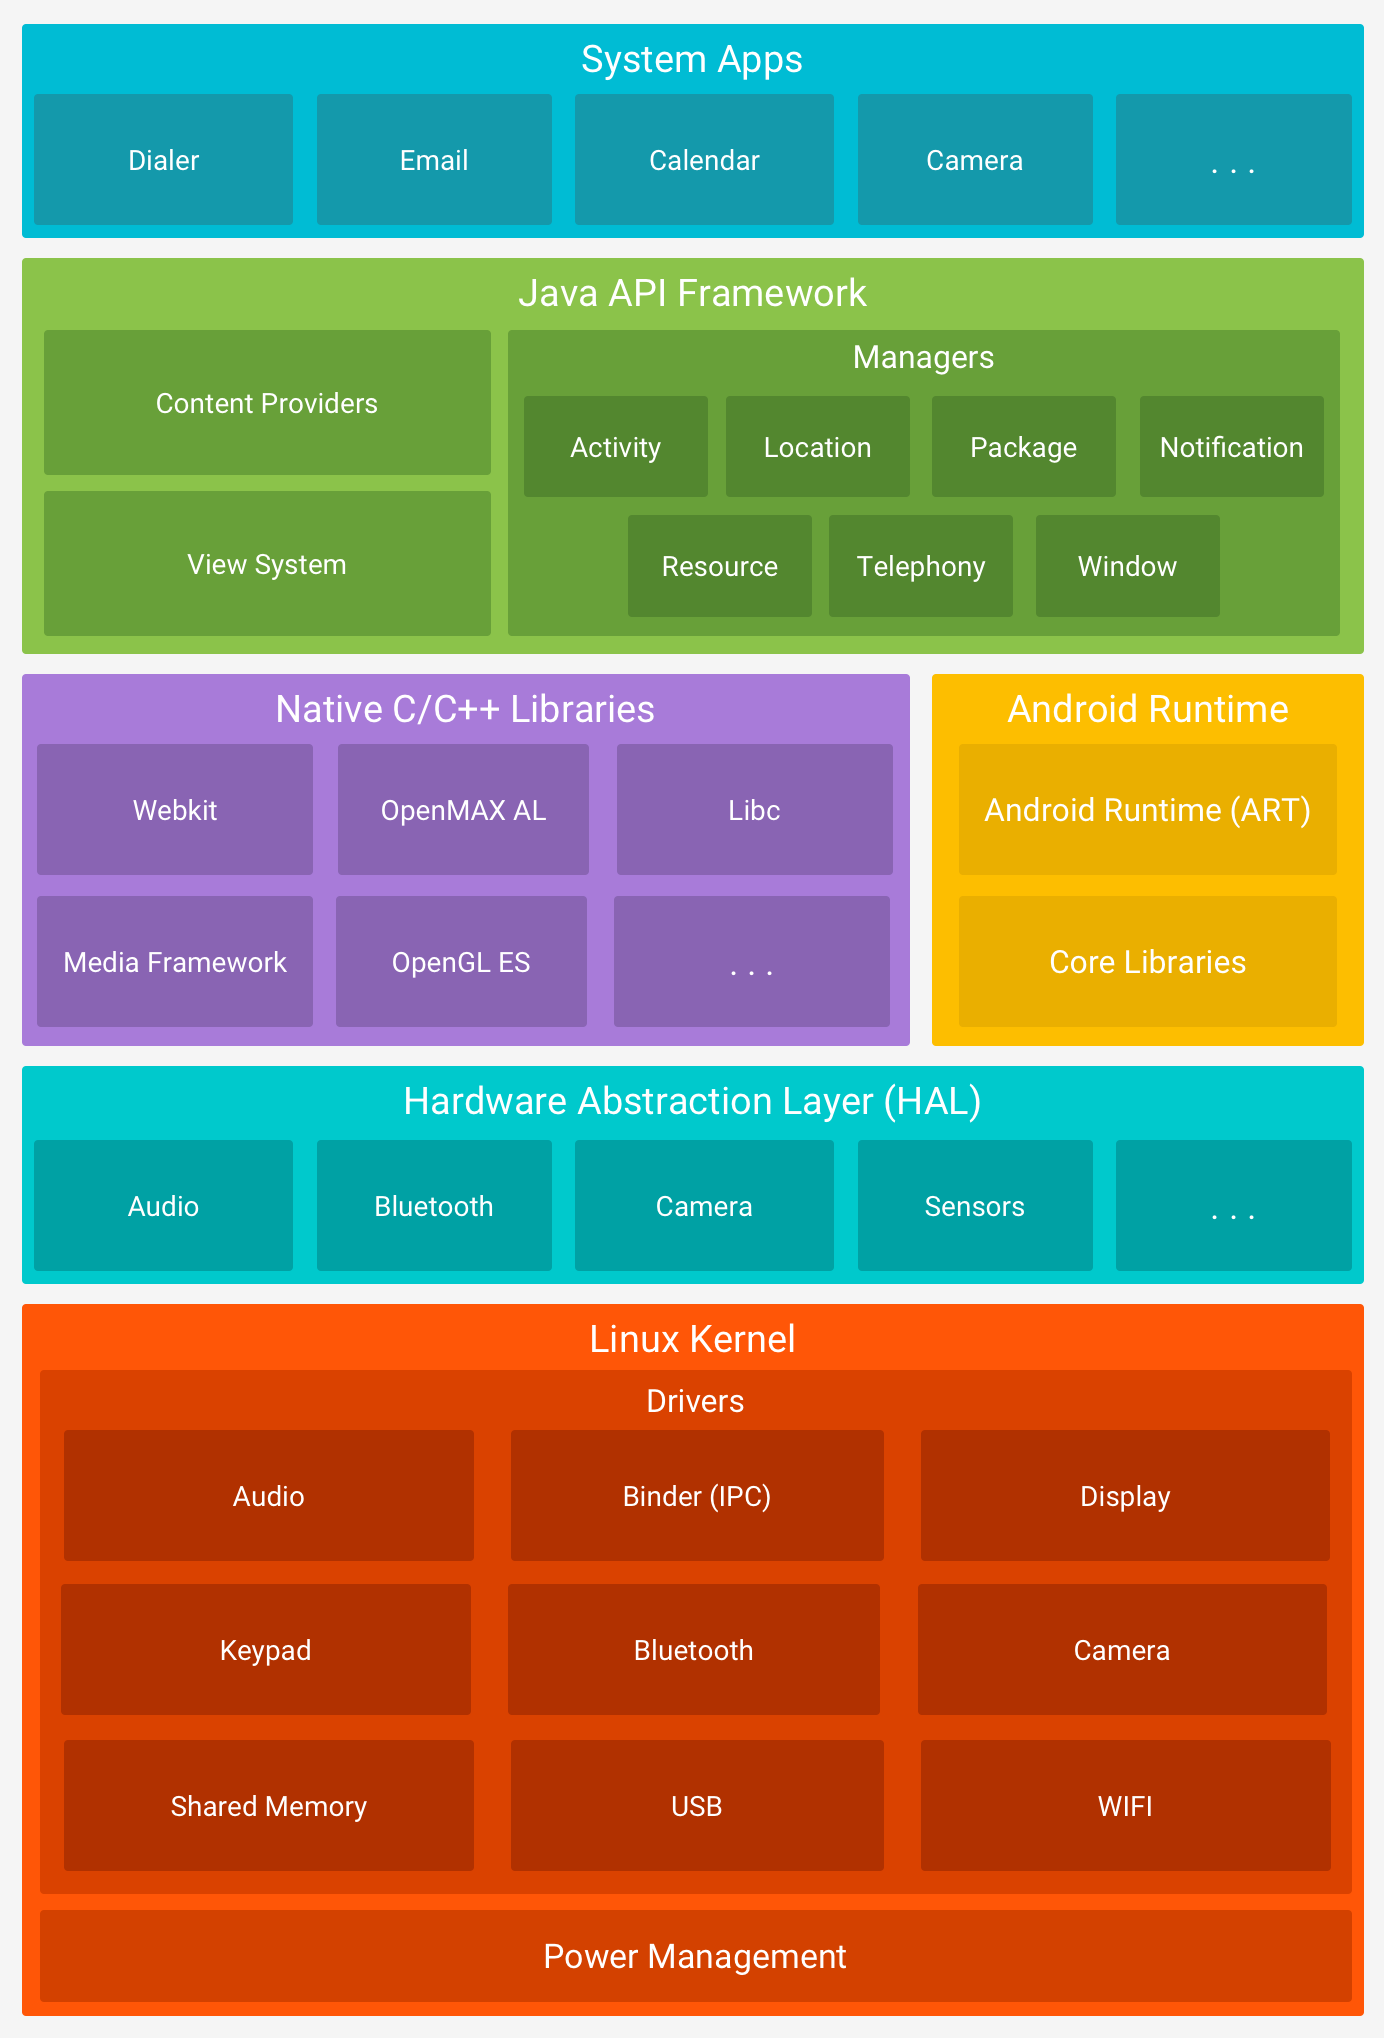
\includegraphics  [scale=0.2,]{img/arq_doc_android.png}}
    \end{frame}
    \label{fig:so_arq_dev_android}
    \source{Retirado de \cite{so_tanembaum}.}
\end{figure}

\newpage

\subsection{Arquitetura de Serviços Mobile}
A Figura \ref{fig:so_arq_android} ilustra a estrutura de processo básica do Android. Em primeiro lugar após o núcleo é o processo \textit{init},o qual gera uma série de processos de \textit{daemon} de baixo nível. Um deles é \textit{zygote}, que é a raiz dos processos de linguagem Java de nível mais alto. O \textit{init} do Android não executa um \textit{shell} da maneira tradicional, já que um dispositivo de Android típico não tem um console local para o acesso do \textit{shell}. Em vez disso, o processo \textit{daemon adbd} executa por conexões remotas que por sua vez  solicitam acesso ao \textit{shell}, criando processos do \textit{shell} para elas conforme a necessidade.

Tendo em vista que a maior parte do Android é escrita na linguagem Java, o \textit{daemon} \textit{zygote} e os processos que ele inicializa são centrais para o sistema. O primeiro processo \textit{zygote} sempre inicia e é chamado de \textit{system\_server} (serviço de sistema), que contém todos os serviços de base do sistema operacional. Partes fundamentais dele são o gerenciador de energia, gerenciador de pacotes, gerenciador de janelas e gerenciador de atividades.
Outros processos serão criados a partir de \textit{zygote} conforme a necessidade.
 
Alguns desses são processos persistentes que fazem parte do sistema operacional básico, como a pilha de telefonia no processo do telefone, que deve permanecer sempre executando. Processos de aplicativos adicionais serão criados e parados conforme a necessidade enquanto o sistema estiver executando.  

%explicar melhor essa figura
 \begin{figure}[htb]
     \caption{Hierarquia de Processos do Android}
     \centering
     \begin{frame}{
     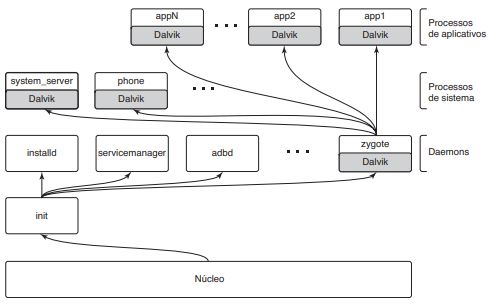
\includegraphics [scale = 1]{img/arquiteturaandroid_tanembaum.JPG}}
     \end{frame}
     \label{fig:so_arq_android}
     \source{Retirado de \cite{so_tanembaum}.}
 \end{figure}

\newpage

\subsection{Linguagem de programação}
Abordando conceitos da cadeira de "Linguagem de Programação III", se faz necessário definir a mesma. Linguagem de programação pode ser definida como uma notação formal e específica para descrever algoritmos para serem executados. Uma linguagem de programação tem dois componentes, sendo esses a Sintaxe e a Semântica. A sintaxe é um conjunto de regras que especificam a composição dos  programas a partir de caracteres. Enquanto isso, as regras de semântica devem especificar o valor de objetos inseridos nos programas \citep{apostila_lp}. 
   
\subsubsection{Dart}

Dart é uma linguagem de programação \textit{open-source} de alto nível desenvolvida pelo Google para desenvolvimento web, criada principalmente com o objetivo de facilitar a criação de aplicações web que acabam sendo muito complexas se feitas a partir dos meios tradicionais, como em linguagens de marcação \citep{dart_walratb_ladd_2012}.% https://dart.dev/mobile  %     [o que é o flutter]

\subsubsection{Flutter}
O Flutter é um framework de desenvolvimento criado pela google para o desenvolvimento de aplicativos mobile híbridos entre Ios E Android. O principal foco do Flutter é tornar o desenvolvimento o mais fácil e produtivo possível, tanto que introduz recursos tais como o \textit{Stateful Hot Reload}, função que permite carregar as alterações para o dispositivo ou emulador sendo usado para visualizar o produto sem precisar compilar todo o aplicativo a cada alteração. Também faz uso de componentes gráficos chamados \textit{Widgets}, os quais também se encontram em vários catálogos \citep{flutter_guide_2019}.

Os Widgets são basicamente componentes de inteface gráfica para o usuário, sendo podem estar organizados em blocos, linhas e colunas. Ao invés de separar as propriedades de componentes em várias \textit{views}, e outras páginas, o flutter apresenta apenas um objeto de modelo, o widget. Os widgets carregam por padrão os estilos \textit{Material}, padrão comum usado em aplicações Android, e \textit{Cupertino}, usado para Ios.

De acordo própria página de visão geral dos aspectos técnicos do Flutter, a mesma diz que o framework é um SDK para criação de aplicativos Android e Ios de alta performance a partir de um único código \citep{tec_ov_flutter}.

A Figura \ref{fig:flutter_layers} ilustra em camadas a base de funcionamento do Flutter. A figura divide em três camadas principais, sendo essas o próprio framework feito com Dart, a Engine, que no caso pode ser o Android Studio, e por último em mais baixo nível a plataforma específica do usuário, cada camada com suas subcamadas.

\begin{figure}[htb]
    \caption{Camadas do Flutter}
    \centering
    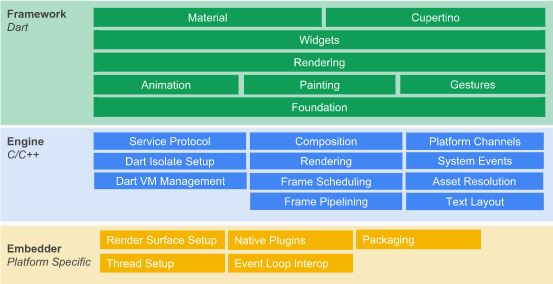
\includegraphics [scale=1.05,]{img/flutter_layers.JPG}
    \label{fig:flutter_layers}
    \source{Adaptado de \cite{tec_ov_flutter}.}
\end{figure}

\newpage

\subsection{Bancos de dados}
Por definição, um banco de dados é um agrupamento de dados que podem ser estabelecidos como o valor de representatividade de algo na vida real. A capacidade dos bancos de dados descende de um corpo de conhecimento e tecnologia que se desenvolveu ao longo de várias décadas e é representado em um software especializado chamado sistema de gerenciamento de banco de dados, ou sistema de banco de dados. Um SGBD provém acesso para criação, manutenção e afins realizados na estrutura e/ou dados inseridos no banco \citep{sbd_korth_silberchatz}.

O sistema de banco de dados é basicamente um sistema de manutenção de registros por computador - ou seja, um sistema cujo objetivo global é manter as informações e torná-las disponíveis quando solicitadas \citep{isbd_cjdate}.

Um banco de dados é uma ferramenta criada com a finalidade de gerenciar dados através de um computador, de forma que os dados nele armazenados mantenham estas informações acessíveis quando necessárias. A manipulação de um banco de dados inclui funções como consulta para recuperar dados específicos, alteração dos dados conforme a demanda e a geração de relatórios com base nos dados gravados \citep{sbd_elmasri_navathe_2011}. 

Os bancos de dados podem ser construídos a partir de um modelo relacional, embasado em um modelo entidade-relacionamento ou também podem ser bancos não relacionais. Nos bancos relacionais, as relações podem ser representadas através de um modelo de tabelas com linhas e colunas, onde as linhas representam um conjunto de valores e as colunas representam qual valor está representado.

\subsubsection{Bancos de dados não relacionais}
No contexto atual, onde um grande volume de dados é gerado a todo momento por diversas aplicações, como redes sociais, há uma grande necessidade para armazenamento e consulta de dados não estruturados, assim havendo um incentivo para o surgimento de novos paradigmas e tecnologias como uma nova categoria de banco de dados, chamada NoSQL (Not Only SQL). Essa tecnologia foi proposta com o objetivo de atender aos requisitos de gerenciamento de grandes volumes de dados, semi-estruturados ou não estruturados, que necessitam de alta disponibilidade e escalabilidade \citep{loscio_oliveira_pontes_nosql_2015}.

Em sua maioria, bancos NoSQL são escritos em JSON, conforme o código 1, adaptado da documentação do Firebase:
\begin{lstlisting}[numbers=left, language=Java, style=mycode, caption={Exemplo de modelagem JSON em Firebase.}, label={lst:firebase-code}]
{
  "usuarios": {
    "jpaulo": {
      "name": "Paulo Jaime",
      "contacts": { "edu": true },
    },
    "edu": { ... },
    "maia": { ... }
  }
}
\end{lstlisting}
\source{Adaptado da documentação do \citet{firebase_docs}.}
\justifying\setlength{\parindent}{1,25cm} 

\subsubsection{Bancos de dados em tempo real}

Sistemas em tempo real podem ser definidos como sistemas para funcionar em um tempo definido. Ou seja, executar certas tarefas com certas restrições de tempo. Portanto, a noção de correção de um sistema em tempo real depende da correção lógica dos resultados produzidos, bem como do momento em que esses resultados são produzidos \citep{realtime_db}.

Um banco de dados em tempo real é simplesmente a integração de um SGBD convencional com um Sistema em Tempo Real. Então, um SGBDTR, além de ser capaz de processar transações e ter a obrigação garantir a integridade e disponibilidade dos dados armazenados, deve trabalhar em tempo real para obedecer as regras de tempo, com as impostas aos sistemas em tempo real. As principais características de um SGBDTR contemplam a noção de dados temporalmente consistentes, e a habilidade para definir restrições temporais às transações \citep{mod_sgbdtr}. 

Ainda conforme dizem \cite{mod_sgbdtr}, observa-se casos em que há restrições temporais que quando impostas às transações precisam ser concluídas com o objetivo de manter a consistência temporal dos dados, ou seja, evitar com que atualizações dessincronizadas possam prejudicar a integridade dos dados. 

\subsubsection{Firebase}
O Firebase é um serviço da \textit{Google Cloud Platform} para prover BaaS e armazenamento de dados, além de oferecer suporte para autenticação de usuários. Quando há integração de um aplicativo com o Firebase, não há necessidade de digitar código back-end ou se preocupar com a estrutura dessa parte do programa \citep{firebase_cheng}.

O \textit{Realtime Database}  do Firebase é um banco de dados não relacional (NoSQL) que permite a distribuição de conteúdos multiplataforma  e com a possibilidade de trabalho offline. Com o Realtime Database não se faz necessária a criação e configuração de servidores ou APIs. É ótimo para validar ideias de apps e soluções web pois não requer manutenção de infra-estrutura \citep{realtime_firebase}.

\pagebreak
A estrutura do banco de dados em firebase se dá por um objeto JSON em hierarquia de árvore, essa estrutura é capaz de suportar diversos tipos de dados. A figura 4 é um exemplo de banco para um app de comércio eletrônico, onde há a produtos e clientes com suas propriedades \citep{firebase_cheng}. 

O Firebase Authentication fornece serviços de back-end e SDKs prontos para autenticar usuários em aplicativos. É oferecido suporte à autenticação através de senhas, números de telefone e até mesmo provedores como Google, Facebook, Twitter entre outros.

Para conectar um usuário a um app, primeiro deve-se ter as credenciais de autenticação do usuário, podendo ser o endereço de e-mail e a senha do usuário ou até mesmo um token de acesso do OAuth de um provedor de identidade federado. Então, são essas credenciais são enviadas para o SDK do Firebase Authentication, onde o back-end faz a  verificação e retorna-se uma resposta ao cliente \citep{firebase_docs}.

Após fazer login, se tem acesso a informações básicas do perfil do usuário e também a capacidade de controlar o acesso do mesmo aos dados armazenados em outros produtos do Firebase. É possível também usar o token de autenticação fornecido para verificar a identidade dos usuários nos seus próprios serviços de back-end \citep{firebase_docs}.

Para o armazenamento de arquivos no firebase usa-se a função de \textit{Cloud Storage}. Com os SDKs do Firebase para Cloud Storage, é permitido fazer \textit{upload} e \textit{download} de arquivos nos aplicativos associados ao Firebase, independentemente da qualidade da rede. Os arquivos são armazenados em um repositório do GCP e são acessados por meio do Firebase. Isso permite executar processos no servidor como filtragem de imagens, vídeo ou outro tipo de documento \citep{firebase_docs}. 

Além disso, o firebase dispõe de uma ferramenta para facilitar o envio de notificações ao usuário através do app, o Firebase Cloud Messaging (FCM). O FCM é uma solução para o envio de mensagens entre plataformas que permite o envio de notificações. A equipe de desenvolvimento pode enviar mensagens de notificação para promover novas interações ou até mesmo tentar influenciar a retenção de usuários. Para casos de uso como mensagens instantâneas, uma mensagem pode transferir um payload de até 4 KB para um app cliente \citep{firebase_docs}.

\subsubsection{GCP - Google Cloud Platform}
O GCP consiste em uma plataforma de acesso a ativos de hardware e software da Google, sendo que esses ativos estão distribuídos em diversos centros da Google pelo mundo. As regiões se dividem em EUA, Europa Ocidental e leste da Ásia, sendo que as mesmas se subdividem em zonas, e a zona, por sua vez, é identificada através de uma nomenclatura que combina um identificador de letra com o nome da região. Como por exemplo, a zona a na região do Leste da Ásia se chama \textit{asia-east1-a}. A distribuição de recursos oferece  vantagens como redundância em caso de falha e também latência reduzida localizando recursos mais próximos de cada cliente, bem como introduz regras sobre como recursos podem ser usados juntos \citep{gcp_2019} .

\subsubsection{Projetos GCP e Firebase}
Para usar ou alocar quaisquer recursos do GCP, é necessário um projeto. Um projeto pode ser pensado como a entidade organizadora do que se está construindo. Um projeto no GCP é feito das configurações, permissões e de outros metadados que descrevem os aplicativos. Os recursos alocados dentro de um único projeto podem funcionar juntos, por exemplo, comunicando-se por meio de uma rede interna. Os recursos usados por cada projeto sempre se mantém separados por limites de projeto entre si, para conectar os mesmos só é possível através de uma rede de internet \citep{gcp_2019}.

Ao criar um novo projeto no Console do Firebase, na verdade está sendo criado um projeto do GCP. É possível fazer a analogia de  um projeto do GCP como um \textit{container} virtual para dados, código, configurações e serviços. Então, um projeto do Firebase é um projeto GCP com configurações e serviços específicos do Firebase. Da mesma forma, também é possível criar um projeto do primeiramente no GCP para depois adicionar o Firebase ao mesmo \citep{firebase_docs}.

Ainda de acordo com a documentação do \citeauthor{firebase_docs}, identifica-se alguns pontos para corroborrar o fato de um projeto do Firebase ser um projeto do GCP, estes são:

\begin{itemize}
    \item Os projetos que aparecem no console do Firebase também aparecem no Console do GCP e no Console de APIs do Google.
    \item O faturamento e as permissões para projetos são compartilhados entre o Firebase e o GCP.
    \item Os identificadores exclusivos de um projeto (como project ID) são compartilhados entre o Firebase e o GCP.
    \itemé possível usar produtos e APIs do Firebase e do GCP no seu projeto.
    \item A exclusão de um projeto o exclui no Firebase e no GCP.
\end{itemize}

\begin{figure}[htb]
     \caption{Visão geral console do projeto no Firebase}
     \centering
     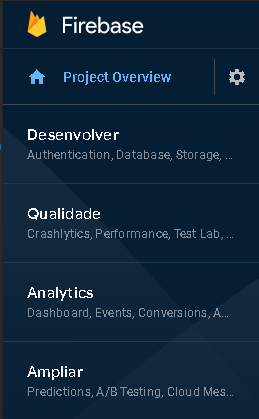
\includegraphics {img/firebase_console.PNG}
     \label{fig:firebase_console}
     \source{Adaptado de \cite{firebase_docs}}   
 \end{figure}
	
Em relação a custos, o Firebase se divide em três planos: \textit{Spark}, \textit{Flame} e \textit{Blaze}, conforme a Figura \ref{fig:firebase_precos}. Como benefício padrão de todos os planos, estão incluídas as funções de análises, notificações, relatórios de erros, suporte e alguns outros.

O \textit{Spark} é o plano gratuito, o mesmo permite o uso limitado das funções de \textit{database, storage, functions, phone auth, hosting} e \textit{test lab}. o Flame é um plano de valor fixo, no valor de US\$ 25,00 por mês e além das funcionalidades do plano \textit{spark}, o flame possui maior espaço disponível no \textit{database} e suporte conexões para o \textit{functions}. Por último, o Blaze, um plano que é pago pela utilização e pode incluir todas as funções do Firebase ao projeto.

\begin{figure}[htb]
    \caption{Planos de preços no Firebase}
    \centering
    \begin{frame}{
    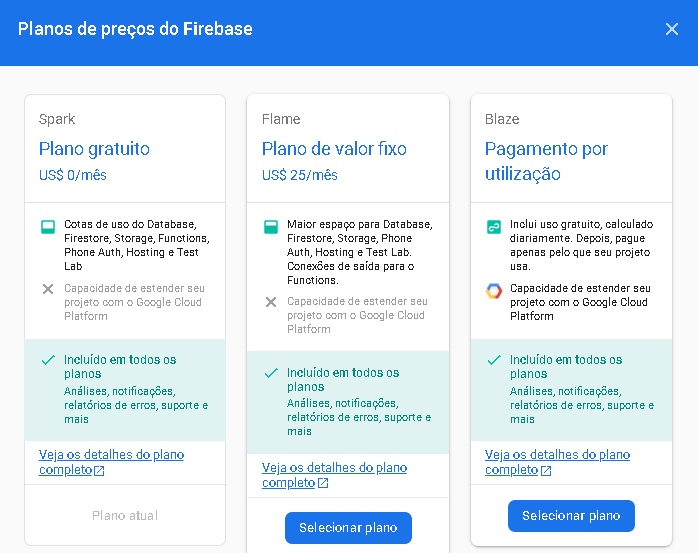
\includegraphics [scale = 0.825]{img/firebase_precos.PNG} }
    \end{frame}
    \label{fig:firebase_precos}
    \source{Retirado de \cite{firebase_docs}}
\end{figure}